

\subsection{Optics}

NIKA2 is a millimeter camera able to simultaneously image a
field-of-view of 6.5arcmin at 150 and 260~GHz, with polarimetric
capabilities at 260~GHz using KIDS. A 30-centimeters diameter air-gap
dichroic splits the 150 GHz (reflection) from the 260 GHz
(transmission) beams.  A grid polarizer ensures then the separation of
the two linear polarisations on the 260 GHz channel.  There are
therefore three KIDS array in NIKA2, one at 2mm, two at 1mm. 


\subsection{Bandpasses {\color{blue} Herv\'e} }


\begin{figure}[ht] % Inline image example
\begin{center}
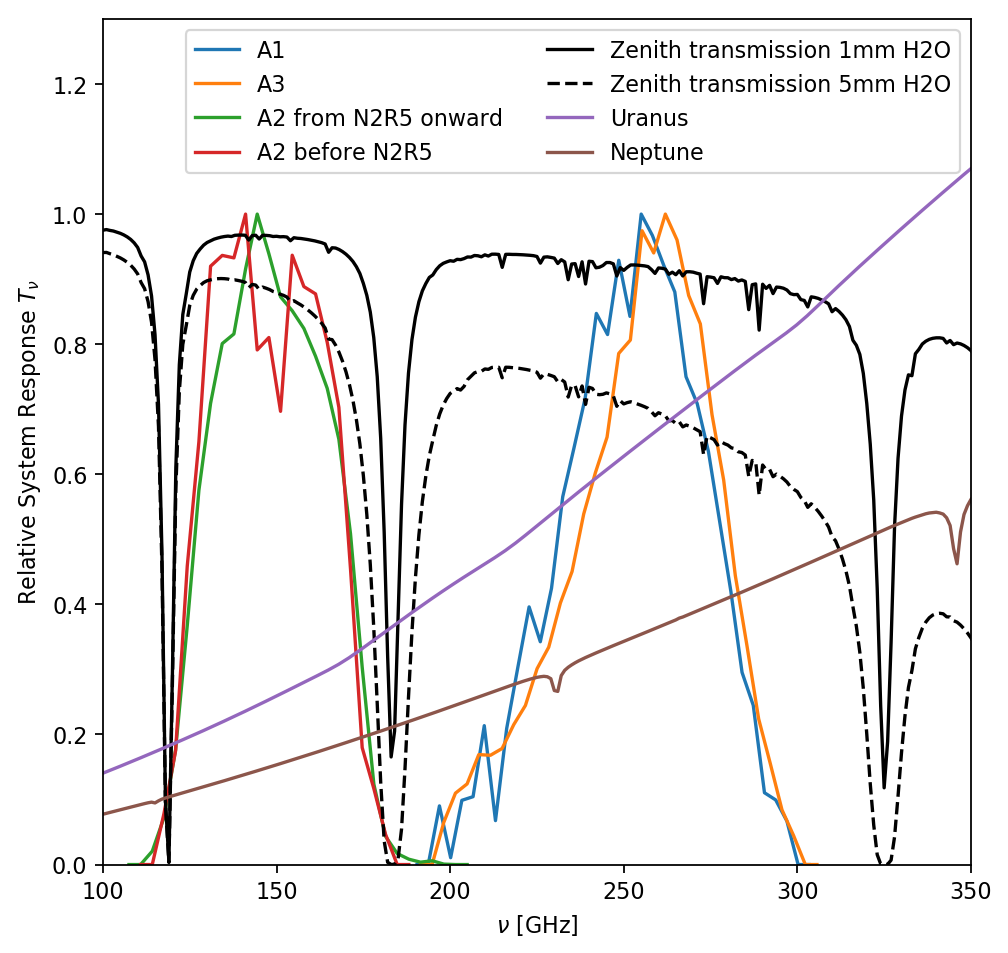
\includegraphics[width=0.9\textwidth]{Figures/SpectralBands/bandpasses_nika2.png}
\caption[NIKA2 transmission]{Relative system response of the three NIKA2 arrays as a
  function of frequency. For illustration we also plot atmospheric transmission obtained with the ATM model 
 \cite{ATM} for different values of precipitable water vapor. The spectra of ESA4 model of Uranus and ESA5 model of Neptune \cite{ESAmodel} in the frequency range are overplotted with arbitrary normalization.} 
 \label{spectralband1}
\end{center}
\end{figure}

 

The NIKA2 spectral bands were measured in the laboratory using a
Martin-Puplett interferometer built in-house \cite{durand}.  Both
arrays and filter bands were considered in the measurements. These
were obtained from the difference of two black bodies, hence they
include a $\nu^2$ Rayleigh-Jeans (RJ) spectral term.
Figure~\ref{spectralband1} shows the relative spectral response for
the three arrays (corrected of the RJ term).  Notice that array A2 was
replaced by a new one in N2R5 and that the spectral transmissions are
not the same (green and red lines in the figure).

The two arrays operating at 260 GHz, mapping different polarisations,
exhibit a slightly different spectral behaviour probably as can be
seen on figure \ref{spectralband1}. This may be explained by a tiny
difference in the silicon wafer and/or Aluminium film thicknesses. For
instance, the observed shift of the peak frequency, 265 GHz for the V
(A1) array versus 258 GHz for the H one (A3), can be explained by
about 5 microns change in the substrate thickness. Hereafter, the peak
frequencies are referred to as reference frequencies (150 and 260 GHz)
to which correpond the reference wavelength (2.0 and 1.15 mm), see
tab.~\ref{tab:nika2summary}.


\begin{table}[th]
\begin{center}
\begin{tabular}{|l|l|r|r|r|r|r|r|}
\hline 
\multirow{3}{*}{Water vapor} & \multirow{3}{*}{Elevation} & \multicolumn{2}{|c|}{1 mm (H)} & \multicolumn{2}{|c|}{1 mm (V)} &
\multicolumn{2}{|c|}{2 mm} \\
 & & $\nu_eff$ & $\Delta \nu$  & $\nu_eff$ & $\Delta \nu$  & $\nu_eff$ & $\Delta \nu$ \\
 & & (GHz) & (GHz)  & (GHz)  & (GHz)   & (GHz)  & (GHz)  \\
\hline
\multicolumn{2}{|c|}{No atmosphere} & 254.71 & 49.21 & 257.39 & 48.05 & 150.93 & 40.72 \\
\hline
\multirow{4}{*}{1 mm $\rm H_2O$ $\rightarrow \tau_{225}=$0.067} & 90 deg &  254.46 & 48.72 & 257.12 & 47.95 & 150.93 & 39.71 \\
 & 60 deg & 254.42 & 48.68 & 257.08 & 47.93 & 150.92 & 39.60 \\
 & 40 deg & 254.33 & 48.57 & 256.98 & 47.89 & 150.88 & 39.32 \\
 & 20 deg & 254.00 & 48.21 & 256.62 & 47.77 & 150.75 & 38.45 \\
\hline
\multirow{4}{*}{2 mm $\rm H_2O$ $\rightarrow \tau_{225}=$0.120} & 90 deg &  254.26 & 48.74 & 256.91 & 48.06 & 150.64 & 39.34 \\
 & 60 deg & 254.20 & 48.70 & 256.84 & 48.07 & 150.60 & 39.19 \\
 & 40 deg & 254.02 & 48.60 & 256.65 & 48.08 & 150.48 & 38.80 \\
 & 20 deg & 253.43 & 48.30 & 256.01 & 47.93 & 150.13 & 37.62 \\
\hline
\multirow{4}{*}{3 mm $\rm H_2O$ $\rightarrow \tau_{225}=$0.173} & 90 deg &  254.06 & 48.76 & 256.70 & 48.19 & 150.39 & 39.03 \\
 & 60 deg & 253.97 & 48.73 & 256.60 & 48.21 & 150.32 & 38.84 \\
 & 40 deg & 253.71 & 48.65 & 256.33 & 48.28 & 150.14 & 38.35 \\
 & 20 deg & 252.86 & 48.41 & 255.40 & 47.86 & 149.60 & 36.94 \\
\hline
\multirow{4}{*}{5 mm $\rm H_2O$ $\rightarrow \tau_{225}=$0.278} & 90 deg &  253.67 & 48.82 & 256.28 & 48.45 & 149.96 & 38.47 \\
 & 60 deg & 253.51 & 48.81 & 256.11 & 48.44 & 149.84 & 38.22 \\
 & 40 deg & 253.10 & 48.77 & 255.68 & 48.26 & 149.54 & 37.58 \\
 & 20 deg & 251.74 & 48.67 & 254.20 & 47.75 & 148.68 & 35.82 \\
\hline
\multirow{4}{*}{8 mm $\rm H_2O$ $\rightarrow \tau_{225}=$0.437} & 90 deg &  253.08 & 48.94 & 255.66 & 48.42 & 149.38 & 37.76 \\
 & 60 deg & 252.84 & 48.93 & 255.39 & 48.35 & 149.20 & 37.42 \\
 & 40 deg & 252.21 & 48.94 & 254.71 & 48.16 & 148.77 & 36.64 \\
 & 20 deg & 250.12 & 49.38 & 252.43 & 47.91 & 147.52 & 34.57 \\
\hline
\multirow{4}{*}{10 mm $\rm H_2O$ $\rightarrow \tau_{225}=$0.542} & 90 deg &  252.70 & 49.00 & 255.24 & 48.38 & 149.04 & 37.34 \\
 & 60 deg & 252.39 & 49.01 & 254.92 & 48.29 & 148.82 & 36.97 \\
 & 40 deg & 251.62 & 49.11 & 254.08 & 48.13 & 148.31 & 36.12 \\
 & 20 deg & 249.07 & 49.75 & 251.28 & 48.24 & 146.85 & 33.93 \\
\hline
\end{tabular}
\caption[Effective frequencies and bandwidthes]{Effective frequencies (for Uranus) and bandwidth of the NIKA2 bands for
  various atmospheric conditions and elevation.}
\label{tab:bandwidths}
\end{center}
\end{table}

%What actually matters more than the ``central frequency'' that depends on many
%assumptions and definitions are the bandpasses. We should make available in a
%.fits file, clearly, our bandpasses to avoid future misunderstanding and propagation of
%false numbers. Official values should be 150 and 260~GHz. We should also clearly
%state that these measured bandpasses were done with the difference of two
%black-bodies, hence they include a $\nu^2$ RJ term.\\

{\color{red} LP: to be moved to Section Calibration ? Opacity ? }


The total system response is the multiplication of the atmospheric
transmission with the relative system response. To derive the
atmospheric transmission, we use GILDAS ATM 2009 model \cite{ATM}, computed for
the IRAM 30-m telescope, with so called {\it midlatwinter} conditions. We select in the model
grid an atmosphere with $T=268.3 \ {\rm K}$ and a pressure of $703.5 \ {\rm hPa}$. The
effective frequency of the passband is defined by:
\begin{equation}
\nu_{eff}( \sec \delta, mm_{H_{2}O}) = \frac{ \int_{0}^{+\infty} S_{\nu}
  T_{\nu}(\sec \delta, mm_{H_{2}O}) \nu d\nu } { \int_{0}^{+\infty} S_{\nu} T_{\nu} d\nu}
\label{eq:nueff0}
\end{equation}

where $T_{\nu}$ is the total system response, normalized between
0. and 1. (i.e. a relative response as a function of the frequency),
hereafter referred to as RSR (Relative System Response), $S_{\nu}$ is
the source spectrum. Table~\ref{tab:bandwidths} list this effective frequency,
computed for Uranus spectrum (ESA4 model, \cite{ESAmodel}), for different atmospheric
water vapor contents and different elevations. 
Table~\ref{tab:bandwidths} also list the bandwidth, defined as:
\begin{equation}
\Delta\nu = \int_{0}^{+\infty} \frac{T_{\nu}}{Max(T_{\nu})}
d\nu
\end{equation}
where the $Max(T_{\nu})$ ensure the RSR span the whole 0.0 to 1.0 range.

From Table~\ref{tab:bandwidths}, we see that the 2 mm band is somewhat
sensitive to the atmospheric conditions, especially at low
elevation. Note that these effective frequencies are {\em not} the
reference frequencies for the band, respectively 150 GHz and 260 GHz
for the A2 and A1, A3 arrays. These reference frequencies are chosen
arbitrarily to define NIKA2 photometric system as will be discussed in section~\ref{se:cal_HA}.

%
% LP: the paragraph below rather belongs to the Opacity section
%
%Using the NIKA2 bandpasses for N2R9, we can integrate the ATM
%atmospheric model to compute the expected ratio between the
%atmospheric opacity of the two NIKA2 channels. 
%Figure~\ref{thopacities} shows the atmospheric opacity
%ratio of the 2 and 1 mm channels as a function of the opacity for the
%1 mm one.

%\begin{figure}[ht] % Inline image example
%\begin{center}
%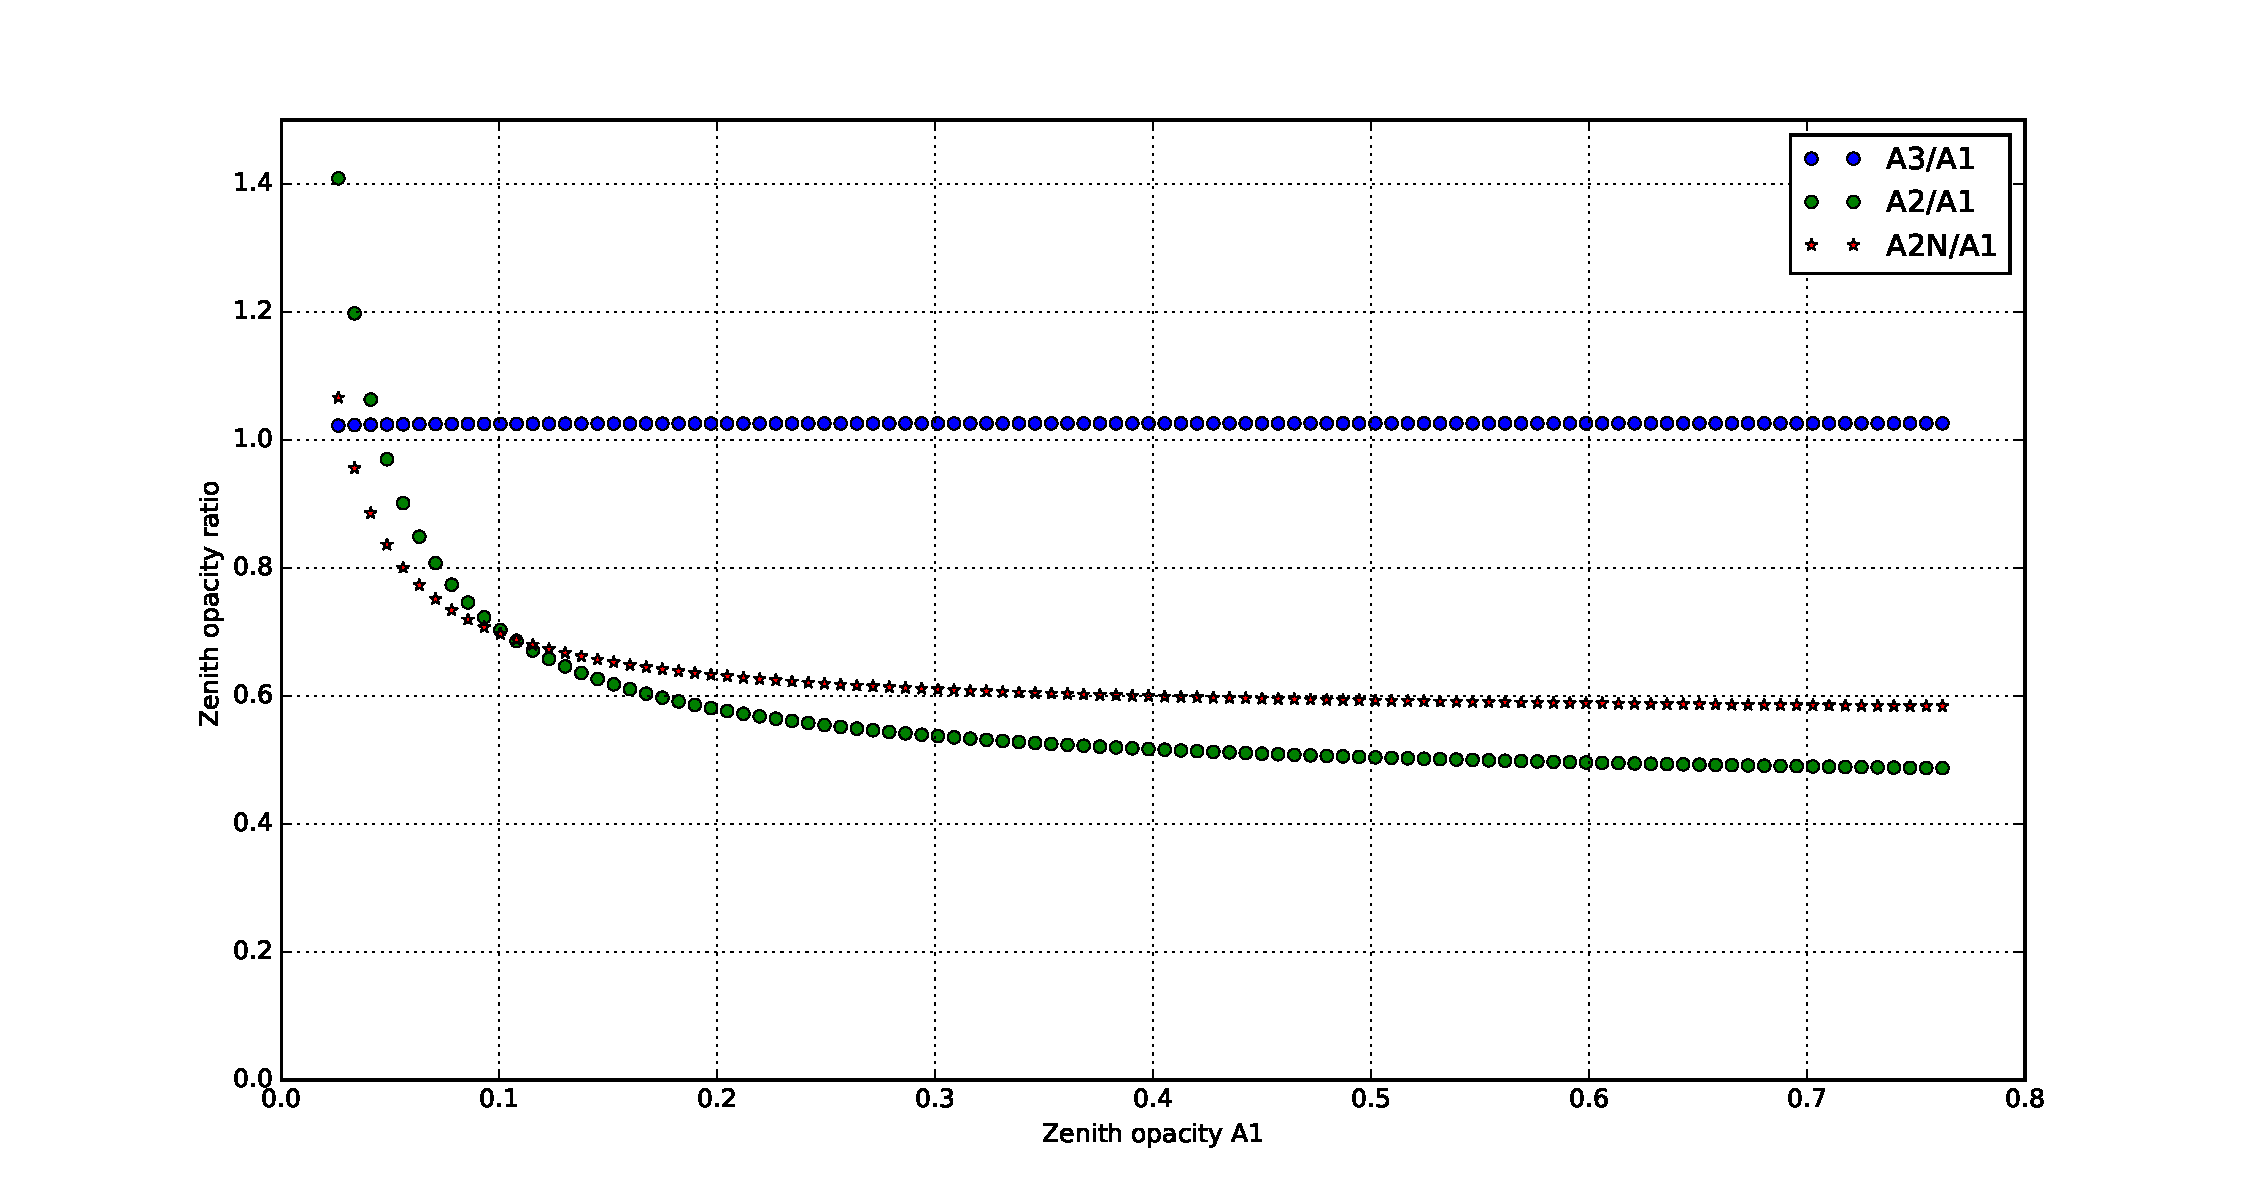
\includegraphics[width=\textwidth]{Figures/SpectralBands/opacity_ratio_vs_tau1.pdf}
%\caption{Expected atmospheric opacity ratio of the 2 and 1 mm channels as function 
%of the opacity at 1 mm. {\bf FM: what is A2N/A1 ?} {\bf FM: why is A3/A1=1 ?}}
%\label{thopacities}
%\end{center}
%\end{figure}




\subsection{Cryogenics}
Further technical details on the NIKA2 instrument can be found in the
technical paper {\bf REF !}



\subsection{KIDs and electronics}

NIKA2 focal plane is equipped with arrays of Kinetic Inductance
Detectors (KIDs hereafter), which are high-quality factor
superconducting resonators. They are operated at 150~mK that is well
below the critical temperature, which ensures their responsivity
properties ... 

\addparag{LUMPED KIDS}

The 2mm array (150~GHz) consist of 616 pixels
(KIDS), disposed to cover a circle with a 78 mm diameter. Each pixel
has a size of $2.8 � 2.8 mm^{2}$ . This is the maximum pixel size that can
be adopted without significantly degrading the telescope resolution,
as it corresponds roughly to a 1F$\lambda$ sampling of the focal
plane.  The array is labelled A2 in all the following.

At 1mm, there are two arrays, labelled A1 and A3, consisting of 1140
KIDS with a size of $2 � 2 mm^{2}$ to ensure a comparable 1F$\lambda$
sampling.


\addparag{NIKEL}


\subsection{KID tuning}

\addparag{$\ftone$ definition}




